\documentclass{article}

\usepackage{amsmath} % math stuff
\usepackage{amssymb} % math stuff
\usepackage{array} % equations and stuff
\usepackage{bm} % bold math
%\usepackage{booktabs} % extra table rule options
%\usepackage{caption} % suppressed table numbering; incompatible with revtex, and longtable, I think
\usepackage{comment} % comment environment
%\usepackage{enumitem} % customization of enumeration, itemize, and description
\usepackage[T1]{fontenc} % font encoding for special characters, must also use scalable font package
\usepackage[margin=0.8in]{geometry} % paper sizes and margins (but be careful not to mess up pre-defined pages)
\usepackage{graphicx} % for graphics
%\usepackage{helvet} % default font is the helvetica postscript font
\usepackage{layouts} % print units like widths
\usepackage{lipsum} % lorem ipsum filler text
\usepackage{lmodern} % scalable font?
\usepackage{longtable} % multi-page tables
\usepackage{makecell} % specify line-breaks in table cells
\usepackage{mathrsfs} % math script font
\usepackage{mhchem} % easier chemical formula
\usepackage{microtype} % allows disabling of ligatures
%\usepackage{newcent} % new century schoolbook font
\usepackage{nicefrac}
\usepackage{numprint} % print and format (large) numbers
\usepackage{parskip} % removes paragraph indentation, and adjusts paragraph skip, as well as list items
\usepackage{pdfpages} % add pdf files as pages
%\usepackage{setspace} % adjust text spacing and indents
\usepackage{siunitx} % decimal alignment
\usepackage{subfigure} % divided figures
%\usepackage{tabu} % extra table options
\usepackage{textcomp} % symbols
\usepackage{threeparttablex} % better footnotes with longtable
\usepackage{titling} % title placement
\usepackage{ulem} % strikethrough text
%\usepackage{url} % superceded by hyperref
\usepackage{verbatim} % verbatim environment
\usepackage{xcolor} % colors and color boxes
\usepackage{xspace} % commands that don't eat up white space
\usepackage{hyperref} % links and page setup; should always come last

\hypersetup{
 bookmarks=true,
 colorlinks=true,
 citecolor=blue,
 linkcolor=blue,
 urlcolor=blue,
 pdfstartview={XYZ null null 1.0} % default open view is 100%
}

\DisableLigatures[f,t]{encoding = T1} % disable ff, fi, fl, tt ligatures; without options, it also disables -- = endash
\renewcommand{\arraystretch}{1.0} % extra vertical (and horizontal?) space in tables

% define centered, left- and right-aligned columns with specified widths
\newcommand{\PreserveBackslash}[1]{\let\temp=\\#1\let\\=\temp}
\newcolumntype{C}[1]{>{\PreserveBackslash\centering}p{#1}}
\newcolumntype{L}[1]{>{\PreserveBackslash\raggedright}p{#1}}
\newcolumntype{R}[1]{>{\PreserveBackslash\raggedleft}p{#1}}

\begin{document}

\pagestyle{empty} % don't number pages

% custom title
\begin{center}
{\LARGE Classic Riddler}

\vspace{0.15in}

{\Large 28 May 2021}
\end{center}


\section*{Riddle:}

Dakota Jones is back in action!
To gain access to a hidden temple deep in the Riddlerian Jungle, she needs a crystal key.

She already knows the crystal is a polyhedron.
And according to an ancient text, it has exactly six edges, five of which are 1 inch long.
Cryptically, the text does not specify the length of the sixth edge.
Instead, it says that the key is the largest such polyhedron (i.e., with six edges, five of which have length 1) by volume.

Once again, Dakota Jones needs your help. What is the volume of the crystal key?


\section*{Solution:}

The only polyhedron with six edges is a tetrahedron, which has four triangular faces.
With five edges of length 1, two of the faces are necessarily equilateral triangles.
These two triangles meet at one edge.
The remaining faces are isosceles (or possibly also equilateral) triangles whose size depend on the length of the last edge.
The length of the last edge is determined by the angle at which the two equilateral faces meet.

I show this in the images below.
On the left is an equilateral triangle, with the perpendicular height $h$ labeled.
On the right is a cross section of the total tetrahedron, with the equilateral faces on the bottom and left.
The two isosceles faces would take up the space shown (with some depth either in or out).
The last edge spans the right side, with the top and right vertices at a distance $h$ from where the equilateral faces meet.

\vspace{0.1in}
\begin{center}
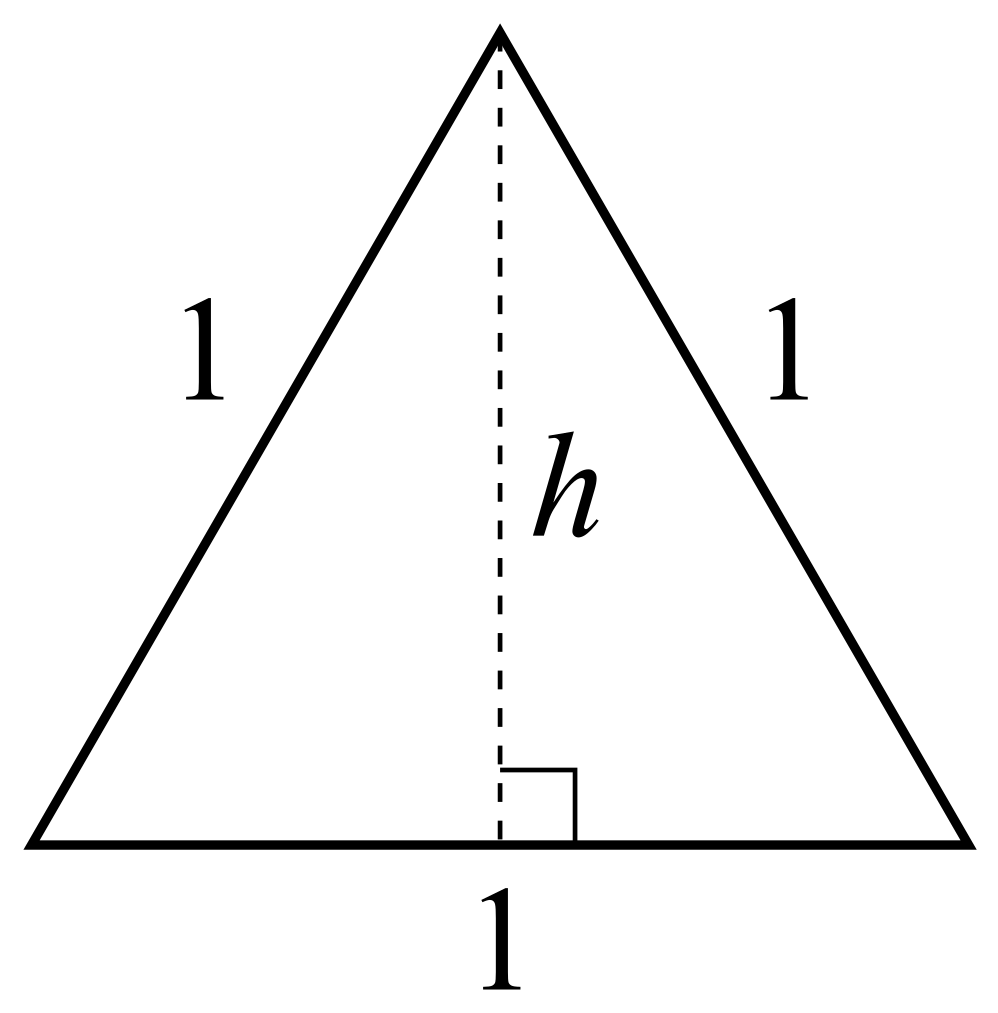
\includegraphics[width=1.75in]{triangle_1.png}
\hspace{1.25in}
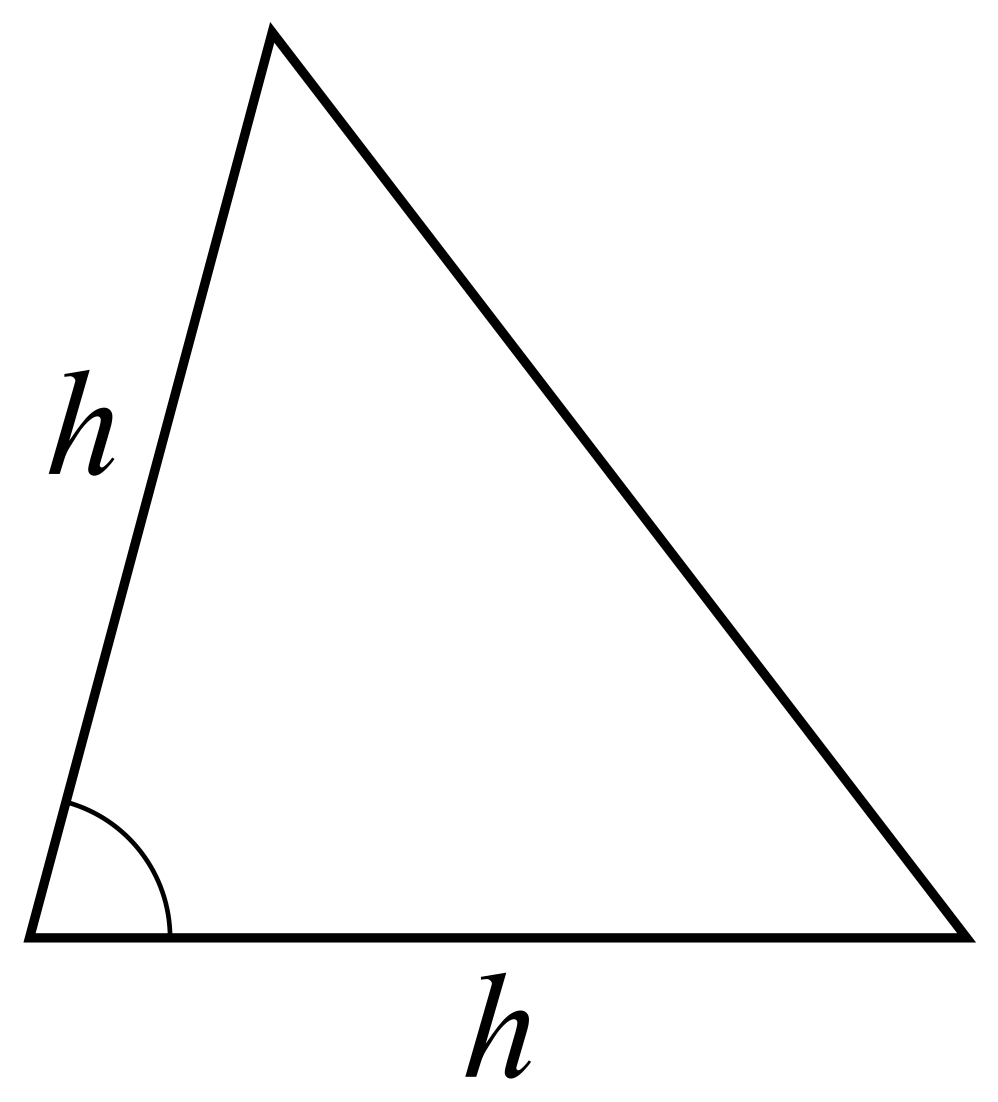
\includegraphics[width=1.75in]{triangle_2.png}
\end{center}
\vspace{0.1in}

The area $A$ of any triangle is $A=\nicefrac{b*h}{2}$, where $b$ is the length of the base.
For the equilateral faces, $b=1$ and $h=\nicefrac{\sqrt{3}}{2}$, so the area is $\nicefrac{\sqrt{3}}{4}$.
The volume $V$ of a tetrahedron can essentially be calculated as the volume of a pyramid: $V=\nicefrac{A*H}{3}$, where $H$ is the height of the pyramid measured from the base with area $A$.

Based on the right drawing above, the volume of the tetrahedron can be calculated with an equilateral triangle as the base.
Then, the volume is maximized when the height $H$ is maximized.
This occurs when the angle between the equilateral faces is 90\textdegree, so that $H=h$.
Plugging in the values above, the volume is
\fcolorbox{red}{white}{$\bm{{\nicefrac{1}{8}}}$}\,.


\end{document}